\chapter{Survival Analysis}
\label{ch-survival}

This chapter is based
on Refs.\cite{lily-xu-284} and \cite{wiki-survival-anal}.

Survival Analysis (SA) is used for curve-fitting, to
fit a curve $S(t)$ to data indicating the number of patients surviving
after receiving a treatment for time $t$.
Alternatively, it can be used with data indicating  the number of
devices that haven't failed after running for time $t$.
SA can also be used  to compare two such $S(t)$ curves---
for example, one for treated patients, and another for non-treated
patients. Hence, SA can be used to analyze the data of an RCT.

Let
\hrule

$\s\in \Sigma$, individual (e.g., patient) in population $\Sigma$.

$N=|\Sigma|$,  size of $\Sigma$, nsam, number of samples

A subset of $\Sigma$, (a.k.a, sub-population
or stratum)
is often called a {\bf cohort}
in epidemiology.

$\tau^\s\geq 0$, time to
{\bf final event} such as death of an organism, or failure
of a device, duration of stay,
follow-up time period,
time period,
lifetime.

$\tau^\s = b^\s -a^\s$ for some absolute times
$a^\s, b^\s$ satisfying
$a^\s<b^\s$

$U^\s=$ {\bf censoring upper bound}

$L^\s=$ {\bf censoring lower bound}

$B^\s = \min(b^s, U^\s)$, {\bf right censoring}

$A^\s = \max(a^s, L^\s)$, {\bf left censoring}

$T^\s = B^\s - A^\s$

$d^\s = \indi(b^\s < U^\s)$, equals 1
if death (i.e., no censoring effect),
equals 0 if no death (i.e., censoring effect)

$e^\s = \indi(a^\s > L^\s)$, equals 1
if death (i.e., no censoring effect),

equals 0 if no death (i.e., censoring   effect)


Will only use right censoring in this chapter.
\hrule
For $t\geq 0$, define
\begin{itemize}
\item {\bf Survival function $S(t)$}
and {\bf Cummulative hazard function $\Lam(t)$}

\beq
S(t) = P(\rvtau > t)= e^{-\Lam(t)}
\eeq
Sometimes, we define $S(t) = P(\rvtau\geq t)$
instead---whatever is more convenient
at the time. For
continuous functions,
these 2 definitions of $S(t)$
are the same.

Note that,
since $S(t)$
is a probability and $t, \tau \in [0, \infty]$, we must have
$\Lambda(t)\geq 0$,
$\Lam(0)=0$ and $\Lam(\infty) = \infty$.

\item {\bf hazard function
(aka , instantaneous failure rate) $\lam(t)$}

\beq
\Lam(t) = \int_0^t  du\; \lam(u)
\eeq

\beq
\lam(t) = \Lam'(t)
\eeq

Note that $\lam(t)\geq 0$
and its integral over $[0,\infty]$
must be $\infty$.
$\lam(t)$ is in fact a conditional probability
as we show next.

\beqa
\lam(t) &=&
\frac{P(\rvtau=t)}{S(t)} \quad \text{(shown below)}
\\
&=&
\frac{P(\rvtau=t)}{P(\rvtau\geq t)}
\\
&=&
\frac{P(\rvtau=t, \rvtau\geq t)}{P(\rvtau\geq t)}
\quad\text{(because $P(A \A B) = P(A)$ if $A$ implies $B$)}
\\
&=&
P(\rvtau=t\cond \rvtau\geq t)
\eeqa


\item {\bf $\rvtau$ density function $P_\rvtau(t)$}

\beq
P_\rvtau(t) = -S'(t) = \lam(t) e^{-\Lam(t)} =
\lam(t)S(t)
\eeq

\item {\bf $\rvtau$ cumulative distribution function
$\Phi_\rvtau(t)$}

\beq
\Phi_\rvtau(t) = P(\rvtau< t) = 1-S(t)
\eeq

\beq
P_\rvtau(t) = \Phi_\rvtau'(t)
\eeq

\item {\bf mean survival time $\mu$}

\beq
\mu= \int_0^\infty dt\; t P_\rvtau(t)
\eeq

\item {\bf median survival time $\tau_{med}$}

\beq
S(\tau_{med})=0.5
\eeq

\end{itemize}

\section{$S(t)$ estimators}

\subsection{No-censoring estimator of $S(t)$}

Let


\beq
r^\s(t) =  \indi(\tau^\s> t)
\eeq
$r^\s(t)$ equals 1 iff individual $\s$
at risk (i.e., still alive
and not censored, not out) at time $t$

\beq
\hat{S}(t) =\frac{1}{N}\sum_\s r^\s(t)
\eeq

$\{\rvr^\s(t):\s\in\Sigma\}$ are i.i.d.

$\rvr^\s(t)=\rvx$ is
a Bernoulli random variable $Bern(p=S(t))$(i.e.,
simple coin flip with $P(\rvx=1)=p$, $P(\rvx=0)=q$,
mean $p$ and variance $pq$, where $p=S(t)$)

\beq
\hat{S}(t)\rarrow
\caln\left(
\mu =S(t), \s^2= \frac{S(t) [1-S(t)]}{N}\right)
\text{ as }N\rarrow \infty
\label{eq-s-est-limit}
\eeq
 (convergence in probability)
A sanity check for Eq.(\ref{eq-s-est-limit}) is to note that

\beqa
\av{\hat{S}(t)}
&=&\frac{1}{N}\sum_\s \underbrace{\av{\rvr^\s(t)}}_{S(t)}
\\
&=&
S(t)
\eeqa


\beqa
\av{\hat{S}(t), \hat{S}(t')}
&=&\frac{1}{N^2}\sum_\s \sum_{\s'}
\av{\rvr^\s(t), \rvr^{\s'}(t')}
\\
&=&
\frac{S(t)[1-S(t)]}{N}
\eeqa

\subsection{Kaplan-Meier estimator of $S(t)$}
Let
\hrule
$[\tau^j[_{j=1,2, \ldots, J}$, times at
which there is an event, all measured
from the same time origin, and
ordered so that $\tau^j < \tau^{j+1}$

$n_D^j=$ number of individuals
that die  at time $\tau^j$


$n_C^j=$ number of individuals
that are censored at time $\tau^j$


$n_O^j=n_D^j+n_C^j$ number of individuals that drop-Out
at time $\tau^j$, either
because they die or are censored


$n_R^j=N-n_O^j$ number of individuals
that are at risk (i.e., still alive
and not censored, not out, surviving) at times $t\geq \tau^j$

\hrule
$d^\s\in\bool$, it equals 1 iff individual
$\s$ dies at any time.

$d^\s(t)\in\bool$, it  equals  1 iff individual
$\s$ dies at time $t$.

$d^\s(\tau^j)\in\bool$, it  equals  1 iff individual
$\s$ dies at time $\tau^j$.

$d^\s(\tau^j)\rarrow \rvd(\tau^j)$ since i.i.d.
\hrule
$c^\s=1-d^\s$, it equals 1 iff individual
$\s$ is censored  at any time.

$c^\s(t)=1-d^\s(t)$, it  equals  1 iff individual
$\s$ is censored at time $t$.

$c^\s(\tau^j)=1-d^\s(\tau^j)$, it  equals  1 iff individual
$\s$ is censored at time $\tau^j$.

$c^\s(\tau^j)\rarrow \rvc(\tau^j)$ since i.i.d.
\hrule

$o^\s(t)=\indi(\tau^\s = t)$, it  equals  1 iff individual
$\s$ drops out at time $t$.

$o^\s(\tau^j)=\indi(\tau^\s = \tau^j)$, it  equals  1 iff individual
$\s$ is drops out at time $\tau^j$.

$o^\s(\tau^j)\rarrow \rvo(\tau^j)$ since i.i.d.
\hrule
Note that\footnote{
notation: $
\A_{i=1,2}a_i = a_1 \A a_2= a_1
\text{ and } a_2\\
\V_{i=1,2}a_i = a_1 \V  a_2 = a_1
\text{ or } a_2\\
\xor_{i=1,2}a_i = a_1 \xor a_2= a_1
\text{ xor } a_2\\
$}

\beq
\underbrace{\bigA_{k\leq j}\{o^\s(\tau^k)=0\}}_{ \text{ $\s$
did not drop out  in past }}=
\underbrace{\bigxor_{k> j}\{o^\s(\tau^k)=1\}}_{ \text{
$\s$ drops out in future }}
\eeq
or, replacing $o^\s$ by $\rvo$,

\beq
\bigA_{k\leq j}\{\rvo(\tau^k)=0\}=
\bigxor_{k> j}\{\rvo(\tau^k)=1\}
\eeq




Kaplan-Meier (KM) estimator of $S(t)$\footnote{Even though $S(t)$ has
been defined as $P(\rvtau>t)$,
a more precise definition
in the presence of censoring is
$P(\rvtau>t|\text{patient dies rather than is censored})$}
\beqa
\hat{S}(\tau^j) &=&
P(\bigxor_{k> j}\{\rvo(\tau^k)=1\})
\\
&=&
P(\bigA_{k\leq j}\{\rvo(\tau^k)=0\})
\\
&=&
\prod_{k\leq j}P(\rvo(\tau^k)=0\cond \bigA_{k'<k}\{\rvo(\tau^{k'})=0\})
\quad \text{(chain rule)}
\\
&=&
\left\{
\begin{array}{l}
\prod_{k\leq j}P(\rvd(\tau^k)=0\cond \bigA_{k'<k}\{\rvo(\tau^{k'})=0\})
\\
+
\underbrace{
\prod_{k\leq j}P(\rvc(\tau^k)=0\cond \bigA_{k'<k}\{\rvo(\tau^{k'})=0\})
}_{=0 \text{(see footnote)}}
\end{array}\right.
\\
&=&
\prod_{k\leq j}\left[1-P(\rvd(\tau^k)=1\cond \bigA_{k'<k}\{\rvo(\tau^{k'})=0\})\right]
\\
&=&
\prod_{k\leq j} \left[ 1 - \frac{n_D^k}{n_R^k}\right]
\eeqa


\begin{figure}[h!]
$$
\xymatrix{
\rvo(\tau^4)
&\rvo(\tau^3)\ar[l]
&\rvo(\tau^2)\ar[l]\ar@/_1pc/[ll]
&\rvo(\tau^1)\ar[l]\ar@/_2pc/[ll]\ar@/_2pc/[lll]
}
$$
\caption{Bnet for KM estimator of $S(t)$
for $N=4$.}
\label{fig-censorless-est}
\end{figure}

Fig.\ref{fig-censorless-est}
gives a bnet for the KM estimator of $S(t)$.
The TPMs, printed in blue, for that bnet,
must be as follows:

\beq \color{blue}
P(\rvo(\tau^k)=1\cond \bigA_{k'<k}\{\rvo(\tau^{k'})=0\})
= \frac{n_O^k}{n_R^k}
\eeq

Intuition:
Let

\beq
\hat{\lam}^k = \frac{n_D^k}{n_R^k}
\eeq
If $\hat{\lam}^k<<1$, then, since
$e^x \approx 1+x $ for $|x|<<1$,

\beqa
\hat{S}(\tau^j) &\approx&
\prod_{k\leq j}e^{\hat{\lam}^k}
\\
&=&
\exp[\sum_{k\leq j}\hat{\lam}^k]
\\
&\approx&
\exp[\int_0^{\tau_j}dt\;\hat{\lam}(t)]
\eeqa
Greenwood's formula
for variance of KM estimator of $S(t)$

\beq
\av{\hat{S}(\tau_j), \hat{S}(\tau_j)}=
[S(t)]^2
\sum_{k\leq j}
\frac{n_D^k}
{ n_C^k n_R^k}
\eeq

Fig.\ref{fig-km-step}
shows relevant parameters
for steps $\tau^{j-1}$ and $\tau^j$
in a plot of a KM estimator.

\begin{figure}[h!]
\centering
\includegraphics[width=3in]
{survival/km-step.png}
\caption{Steps $\tau^{j-1}$ and $\tau^j$
in a plot of a KM estimator. An ${\bf X}$ indicates a dead individual
and $\blacksquare$ a censored one.
Note that\\
$n_O^j= n_D^j+n_C^j$, \\
$n_R^j = n_R^{j-1} - n_O^{j-1}(t)$
and\\
$n_R^j = \sum_{k\geq j} n_O^k$.}
\label{fig-km-step}
\end{figure}

Fig.\ref{fig-kn-graph} gives a numerical
example of the
 KM estimator.

 \begin{figure}[h!]
\centering
\includegraphics[width=4in]
{survival/km-graph.png}
\begin{tabular}{|c|c|c|c|c|c|c|}
\hline\hline
6& 6& 6& 6C& 7& 9C& 10\\
\hline
10C&11C& 13& 16& 17C& 19C& 20C\\
\hline
 22& 23& 25C& 32C& 32C& 34C& 35C\\
 \hline
 \end{tabular}
\caption{Plot of KM estimator for
$N=21$ patients
with $\tau^\s$ given in table
below the graph.
$\tau's$ with $C$
 are censored.}
\label{fig-kn-graph}
\end{figure}





\section{$\lam(t)$ models}

\subsection{$\lam(t)$  independent
of covariates $z$}

recall $t\geq 0$
\begin{itemize}
\item $\lam$ independent of time

\beq
\lam(t) = \lambda
\eeq
where $\lam \geq 0$.

\beq
\Lambda(t) = \lam t
\eeq

\beq
P_\rvtau(t) = \lam e^{-\lam t}
\quad\text{(Exponential distribution)}
\eeq

\item  $\lam$ proportional to power of $t$

\beq
\lam(t) = \kappa\lam t^{\kappa-1}
\eeq
where $\lam, \kappa\geq 0$.

\beq
\Lambda(t) = \lam t^\kappa
\eeq

\beq
P_\rvtau(t)=\kappa\lam t^{\kappa-1} e^{-\lam t^\kappa}
\quad \text{(Weibull  distribution)}
\eeq

\item $\lam(t)= a + bt$ for $a,b\geq 0$

\item $\lam(t)$ piecewise constant for $t\in [0, \infty]$


\item etc.

\end{itemize}


\subsection{$\lam(t)$  dependent
of covariates $Z$}

Suppose $\beta, Z\in \RR^{nind}$ are
column vectors, where $nind$ is
number of independent variables (covariates)
in a regression.

{\bf Cox Proportional Hazards (PH) model for
$\lam(t)$}

\beq
\lam(t) =\lam(t|Z) = \lam_0(t) e^{\beta^T Z}
\eeq
where $\lam_0(t)\geq 0$.
$\lam_0(t)$
is called the {\bf baseline
hazard function}.
This $\lam(t)$  model is called a
PH model because
$\lam(t|Z_1)/\lam(t|Z_2)=
\exp[\beta^T(Z_1-Z_2)]$
is independent of time.

Note that since exponentials
are always positive, the components
of $\beta$ and $Z$ can
range over all real values.
If we had chosen
$\lam(t) = \lam_0(t)\beta^T Z$
instead, then we would have
to constrain $\beta^TZ\geq 0$.

If we define

\beq
\Lambda_0(t) = \int_0^t du\;\lam_0(u)
\eeq
then

\beq
P_\rvtau(t) =\lam_0(t) e^{\beta^T Z} \exp[-\Lam_0(t)
e^{\beta^T Z}]
\eeq
$P_\rvtau(t)$ is called the {\bf Cox PH distribution}.
It's a {\bf semi-parametric distribution}
because it depends on both, a prior
parameter $\beta$ and a prior function $\lam_0(t)$
(a function is like an infinite dimensional parameter).
A {\bf parametric  distribution}
depends only on a prior parameter and
a {\bf non-parametric  distribution}
depends only on a prior function.

Recall that we defined earlier

$n_D^j=$ number of individuals
that die  at time $\tau^j$


$n_C^j=$ number of individuals
that are censored at time $\tau^j$


$d^\s\in \bool$, it equals 1 iff individual
$\s$ dies at any time.

$c^\s= 1-d^\s$, it equals 1 iff individual
$\s$ is censored at any time.

To define the Cox partial likelihood function,
we will assume that $n^j_D + n^j_C =1$, i.e.,
each time $\tau^j$ has either
a single death, or a single censorship, but not both.
Since every individual
eventually dies or is censored (but, we will assume, not both),
there is a 1-1 onto map $j(\s)$ mapping $\Sigma$ to the set
of indices of $\tau^j$. So we can label the population individuals by
the index $j(\s)$.

Let

\beq
\call^j (\beta)=
\frac{ e^{\beta^T Z^j}}
{\sum_{k\geq j} e^{\beta^T Z^{k}}}
\eeq
Then define the {\bf Cox partial likelihood function} by


\beq
\call(\beta) = \prod_j [\call^j(\beta)]^{d^j}
\eeq
Cox's approximate method for finding
the best fit for $\beta$
is to set $
\pder{\call(\beta)}{\beta_a} =0$
for all $a$. This does not determine the
baseline hazard function, however.

Recall that

\beq
\lam(\tau^{j}|Z^{k})=
\lam_0(\tau^{j})e^{\beta^T Z^{k}}
=
P(\rvtau^k=\tau^j\cond \rvtau^k\geq \tau^j)
\eeq
Therefore

\beqa
\call^j (\beta)
&=&
\frac{ \lam_0(\tau^{j})e^{\beta^T Z^j}}
{\sum_{k\geq j}\lam_0(\tau^{j}) e^{\beta^T Z^{k}}}
\\
&=&
\frac{ \lam(\tau^{j}|Z^j)}
{\sum_{k\geq j}\lam(\tau^{j}|Z^{k})}
\eeqa


Next, we try to justify Cox's partial likelihood
function.
We will give two arguments.

\begin{enumerate}
\item Bayesian argument

Assume that $Z^{k}$ is a random variable
with a non-informative prior $P(Z^{k})=\caln(!k)$.
Then

\beq
P(Z^{k}|\tau^{j}) = f(\tau^j)\underbrace{P(\tau^j|Z^{k})}_
{\lam(\tau^j|Z^{k})}
\eeq
for some function $f:\RR\rarrow \RR$.
Hence

\beqa
\call^j (\beta)&=&
\frac{ P(Z^j\cond\tau^{j})}
{\sum_{k\geq j}P(Z^{k}\cond\tau^{j})}
\\
&=&
\frac{ P(Z^j\cond\tau^{j})}
{P(\bigxor_{k\geq j}\{\ul{Z}^{k}=Z^k\}\cond\tau^{j})}
\quad\text{(because the $Z^k$ are independent)}
\\
&=&
\frac{ P(Z^j,\bigxor_{k\geq j}\{\ul{Z}^{k}=Z^k\},\tau^{j})}
{P(\bigxor_{k\geq j}\{\ul{Z}^{k}=Z^k\},\tau^{j})}
\\
&=&
P(Z^j\cond \bigxor_{k\geq j}\{\ul{Z}^{k}=Z^k\},\tau^{j})
\eeqa

Note that $\call^j(\beta)$ depends
on $\{Z^k: k\geq j\}$ because at time $j$,
the past $Z^k$ are fixed already,
so the only ones we are allowed
to optimize (remember, we are acting as
Bayesians here, so we can  optimize parameters)
 are the future ones.
\item Maximum Likelihood argument

\beqa
\call^j(\beta)&=&
\left\{
\begin{array}{ll}
P(\rvtau>\tau^j) =S(\tau^j)
& \text{ if $d(\tau^j)=0$ so $c(\tau^j)=1$}
\\
 P(\rvtau=\tau^j)=
 \lam(\tau^j\cond Z^j) S(\tau^j)
  & \text{ if $d(\tau^j)=1$ }
 \end{array}\right.
 \\
 &=&
 \lam(\tau^j\cond Z^j)^{d(\tau^j)} S(\tau^j)
 \\
 &=&
\underbrace{\left[\frac{\lam(\tau^j\cond Z^j)}
{\sum_{k\geq j} \lam(\tau^k\cond Z^j)}
\right]^{d(\tau^j)}
}_{L_1}
\underbrace{
\left[
\sum_{k\geq j} \lam(\tau^k\cond Z^j)
\right]^{d(\tau^j)}
S(\tau^j)
}_{L_2}
\eeqa
Cox argued that $L_2$ varies very slowly
with $\beta$.
\end{enumerate}


\section{$S_0(t)$ estimators}

\beqa
S_Z(t)&=&
e^{-\Lam(t)}
\\
&=&
e^{-\Lam_0(t)\exp(\beta^TZ)}
\\
&=&
S_{Z=0}(t)^{\exp(\beta^TZ)}
\eeqa

\begin{claim}(Breslow $S_0(t)$ estimator)

\beq
\hat{S}_0(t)= e^{-
\hat{\Lam}_0(t)}
\eeq
where

\beq
\hat{\Lam}_0(t)=
\sum_{j: \tau^j<t}
\left[
\frac{n_D^j}
{\sum_{k\geq j} e^{\beta^TZ^k}
}
\right]
\label{eq-breslow}
\eeq


\end{claim}
\proof

\beqa
\frac{n_D^j}{\Delta t}
&\approx&
\sum_{k\geq j}
P(\rvtau^k=\tau^j\cond \rvtau^k>\tau^j)
\\
&=&
\sum_{k\geq j}
\lam(\tau^j\cond Z^k)
\\
&=&
\lam_0(\tau^j)
\sum_{k\geq j}
e^{\beta^TZ^k}
\eeqa
Hence
\beq
\lam_0(t)\Delta t=
\frac{n_D^j}
{\sum_{k\geq j} e^{\beta^TZ^k}}
\eeq
If we now apply
$\sum_{j: \tau^j<t}$ to both
sides of the last equation, we get Eq.(\ref{eq-breslow}).
\qed

Note that

\beqa
\hat{S}_0(t)
&=&
\prod_{j: \tau^j<t}
\exp
\left[
\frac{-n_D^j}
{\sum_{k\geq j} e^{\beta^TZ^k}
}
\right]
\\
&\approx&
\prod_{j: \tau^j<t}
\left[1-
\underbrace{\frac{n_D^j}
{\sum_{k\geq j} e^{\beta^TZ^k}
}}_{\hat{\lam}^j}
\right]
\text{(because $e^x\approx 1 + x$ for $|x|<<1$)}
\eeqa
